\chapter{Spendley's et al. method}

In this chapter, we present Spendley's et al. algorithm \cite{Spendley1962} for 
unconstrained optimization.

We begin by presenting a global overview of the algorithm. 
Then we present various geometric situations which might occur
during the algorithm. In the second section, we present several 
numerical experiments which allow to get some insight in the behaviour 
of the algorithm on some simple situations. The two first cases 
are involving only 2 variables and are based on a quadratic function.
The last numerical experiment explores the behaviour of the algorith
when the number of variables increases.

\section{Introduction}

In this section, we present Spendley's et al algorithm for unconstrained optimization.
This algorithm is based on the iterative update of a simplex. 
At each iteration, either a reflection of a shrink step is performed, so that
the shape of the simplex does not change during the iterations.
Then we present various geometric situations which might occur
during the algorithm. This allows to understand when exactly a reflection 
or a shrink is performed in practice.

\subsection{Overview}

The goal of Spendley's et al. algorithm is to solve the 
following unconstrained optimization problem
\begin{eqnarray}
\min f(\bx)
\end{eqnarray}
where $\bx\in \RR^n$, $n$ is the number of optimization parameters and $f$ is the objective 
function $f:\RR^n\rightarrow \RR$.

The simplex algorithms are based on the iterative update of 
a \emph{simplex} made of $n+1$ points $S=\{\bx_i\}_{i=1,n+1}$. Each point 
in the simplex is called a \emph{vertex} and is associated with 
a function value $f_i=f(x_i)$ for $i=1,n+1$.

The vertices are sorted by increasing function values so that the 
\emph{best} vertex has index 1 and the \emph{worst} vertex 
has index $n+1$
\begin{eqnarray}
\label{sorted-vertices-fv}
f_1 \leq f_2 \leq \ldots \leq f_n \leq f_{n+1}.
\end{eqnarray}

The $\bx_1$ vertex (resp. the $\bx_{n+1}$ vertex) is called the \emph{best} 
vertex (resp. \emph{worst}), because it is associated with the lowest (resp. highest)
function value. As we are going to see, the \emph{next-to-worst} vertex $\bx_n$ has a 
special role in this algorithm.

The centroid of the simplex $\overline{\bx} (j)$ is the center of the vertices
where the vertex $\bx_j$ has been 
excluded. This centroid is 
\begin{eqnarray}
\label{centroid-generalized}
\overline{\bx} (j) = \frac{1}{n} \sum_{i=1,n+1, i\neq j} \bx_i.
\end{eqnarray}
The algorithm makes use
of one coefficient $\rho>0$, called the reflection factor. The standard
value of this coefficient is $\rho=1$.
The algorithm attemps to replace some vertex 
$\bx_j$ by a new vertex $\bx(\rho,j)$ on the line from the vertex $\bx_j$
to the centroid  $\overline{\bx}(j)$. The new vertex $\bx(\rho,j)$ is defined by 
\begin{eqnarray}
\label{interpolate-generalized}
\bx(\rho,j) = (1+\rho)\overline{\bx}(j) - \rho \bx_j.
\end{eqnarray}

\subsection{Algorithm}

The first step of the algorithm is based on the centroid 
where the worst vertex $\bx_{n+1}$ has been excluded. This centroid 
$\overline{\bx} (n+1)$ is 
\begin{eqnarray}
\label{centroid-worst}
\overline{\bx} (n+1) = \frac{1}{n} \sum_{i=1,n} \bx_i.
\end{eqnarray}
This step is a reflection with respect to the worst vertex $\bx_{n+1}$ so that the 
reflected point $\bx_r$ is defined by 
\begin{eqnarray}
\label{interpolate-worst}
\bx_r = \bx(\rho,n+1) = (1+\rho)\overline{\bx}(n+1) - \rho \bx_{n+1}
\end{eqnarray}

We then compute the function value of the reflected
point $f_r=f(\bx_r)$. If the function value $f_r$ is better than the worst function
value $f_{n+1}$, i.e. if $f_r < f_{n+1}$, then the worst point $\bx_{n+1}$ is rejected from the 
simplex and the reflected point $\bx_r$ is accepted. If the reflection point 
does not improve the function value $f_{n+1}$, we consider the centroid 
$\overline{\bx} (n)$, i.e. the centroid where the vertex $\bx_n$ has been excluded.
We then consider the reflected vertex $\bx_r^\prime$, computed from the 
next-to-worst vertex $\bx_n$ and the centroid $\overline{\bx} (n)$. 
We compute the function value $f_r^\prime = f(\bx_r^\prime)$. If the function
value $f_r^\prime$ improves over the worst function value $f_{n+1}$, the new reflection vertex 
$\bx_r^\prime$ is accepted.

At that point of the algorithm, neither the reflection with respect to 
$\bx_{n+1}$ nor the reflection with respect to $\bx_n$ were able to improve over 
the worst function value $f_{n+1}$.
Therefore, the algorithm shrinks the simplex toward the best vertex $\bx_1$.
That last step uses the shrink coefficient $0<\sigma<1$. The standard
value for this coefficient is $\sigma=\frac{1}{2}$.

Spendley's et al. algorithm is presented in figure \ref{algo-spendley}.

\begin{figure}[htbp]
\begin{algorithmic}
\STATE Compute an initial simplex $S_0$
\STATE Sorts the vertices $S_0$ with increasing function values
\STATE $S\gets S_0$
\WHILE{$\sigma(S)>tol$}
  \STATE $\overline{x}\gets \overline{x}(n+1)$
  \STATE $x_r \gets x(\rho,n+1)$, $f_r \gets f(x_r)$ \COMMENT{Reflect with respect to worst}
  \IF {$f_r<f_{n+1}$}
    \STATE Accept $x_r$
  \ELSE
    \STATE $\overline{x}\gets \overline{x}(n)$
    \STATE $x_r \gets x(\rho,n)$, $f_r \gets f(x_r)$ \COMMENT{Reflect with respect to next-to-worst}
    \IF {$f_r<f_{n+1}$}
      \STATE Accept $x_r$
    \ELSE 
      \STATE Compute the points $x_i=x_1 + \sigma (x_i - x_1)$, $i=2,n+1$ \COMMENT{Shrink}
      \STATE Compute the function values at the points $x_i, i=2,n+1$
    \ENDIF
  \ENDIF
  \STATE Sort the vertices of $S$ with increasing function values
\ENDWHILE
\end{algorithmic}
\caption{Spendley et al. algorithm}
\label{algo-spendley}
\end{figure}

\subsection{Geometric analysis}

The figure \ref{fig-spendley-moves} presents the various 
moves of the Spendley et al. algorithm. It is obvious from the 
picture that the algorithm explores a pattern which is 
entirely determined from the initial simplex.

\begin{figure}
\begin{center}
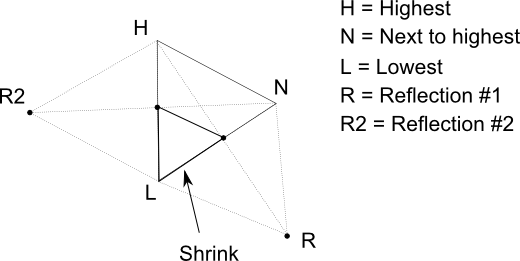
\includegraphics[width=10cm]{spendley-steps.png}
\end{center}
\caption{Spendley et al. simplex moves}
\label{fig-spendley-moves}
\end{figure}

The various situations in which these moves are performed are 
presented in figures \ref{fig-spendley-moves-reflect}, \ref{fig-spendley-moves-reflect2}
and \ref{fig-spendley-moves-shrink}.

The basic move is the reflection step, presented in figure 
\ref{fig-spendley-moves-reflect} and \ref{fig-spendley-moves-reflect2}. 
These two figures shows that the Spendley et al.
algorithm is based on a discretization of the parameter space. 
The optimum is searched on that grid, which is based on regular simplices.
When no move is possible to improve the situation on that grid,
a shrink step is necessary, as presented in figure \ref{fig-spendley-moves-shrink}.

\begin{figure}
\begin{center}
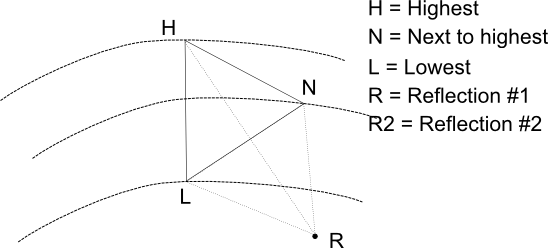
\includegraphics[width=10cm]{spendley-steps-reflect.png}
\end{center}
\caption{Spendley et al. simplex moves -- Reflection with respect to highest point}
\label{fig-spendley-moves-reflect}
\end{figure}

\begin{figure}
\begin{center}
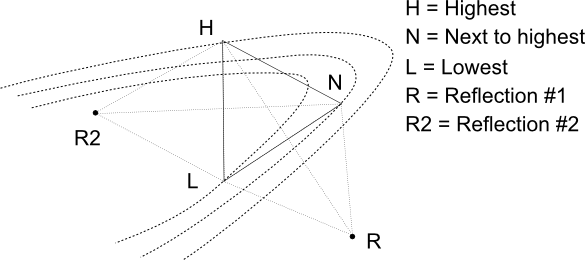
\includegraphics[width=10cm]{spendley-steps-reflect2.png}
\end{center}
\caption{Spendley et al. simplex moves -- Reflection with respect to next-to-highest point. 
It may happen that the next iteration is a shrink step.}
\label{fig-spendley-moves-reflect2}
\end{figure}

In the situation of figure \ref{fig-spendley-moves-shrink}, neither the 
reflection \#1 or reflection \#2 have improved the simplex. 
Diminishing the size of the simplex by performing a shrink step 
is the only possible move because the 
simplex has vertices which are located across the valley.
This allows to refine the discretization grid on which the 
optimum is searched.

\begin{figure}
\begin{center}
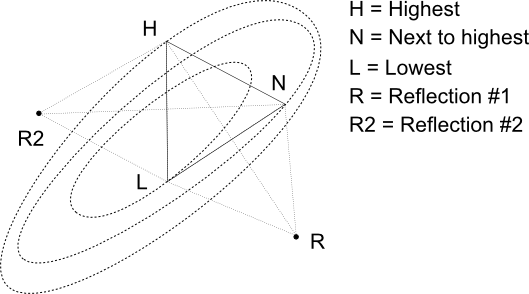
\includegraphics[width=10cm]{spendley-steps-shrink.png}
\end{center}
\caption{Spendley et al. simplex moves -- Shrink.}
\label{fig-spendley-moves-shrink}
\end{figure}

%% \subsection{Termination criteria}

%% TODO...

%% \subsection{General features of the algorithm}

%% TODO...


\section{Numerical experiments}

In this section, we present some numerical experiments 
with the Spendley et al. algorithm.

\subsection{Quadratic function}

The function we try to minimize is the following quadratic 
in 2 dimensions 

\begin{eqnarray}
f(x_1,x_2) = x_1^2 + x_2^2 - x_1 x_2
\end{eqnarray}

The stopping criteria is based on the relative size of the simplex 
with respect to the size of the initial simplex 

\begin{eqnarray}
\sigma(S) < tol \times \sigma(S_0)
\end{eqnarray}

The initial simplex is a regular simplex with length unity.

The following Scilab script performs the optimization.

\lstset{language=scilabscript}
\begin{lstlisting}
function y = quadratic (x)
  y = x(1)^2 + x(2)^2 - x(1) * x(2);
endfunction
nm = neldermead_new ();
nm = neldermead_configure(nm,"-numberofvariables",2);
nm = neldermead_configure(nm,"-function",quadratic);
nm = neldermead_configure(nm,"-x0",[2.0 2.0]');
nm = neldermead_configure(nm,"-maxiter",100);
nm = neldermead_configure(nm,"-maxfunevals",300);
nm = neldermead_configure(nm,"-tolxmethod","disabled");
nm = neldermead_configure(nm,"-tolsimplexizerelative",1.e-8);
nm = neldermead_configure(nm,"-simplex0method","spendley");
nm = neldermead_configure(nm,"-method","fixed");
nm = neldermead_configure(nm,"-verbose",1);
nm = neldermead_configure(nm,"-verbosetermination",0);
nm = neldermead_search(nm);
neldermead_display(nm);
nm = neldermead_destroy(nm);
\end{lstlisting}


The numerical results are presented in table \ref{fig-spendley-numexp1-table}.

\begin{figure}[htbp]
\begin{center}
\begin{tiny}
\begin{tabular}{|l|l|}
\hline
Iterations & 49 \\
Function Evaluations & 132 \\
$x_0$ & $(2.0,2.0)$ \\
Relative tolerance on simplex size & $10^{-8}$ \\
Exact $x^\star$ & $(0.,0.)$\\
Computed $x^\star$ & $(2.169e-10, 2.169e-10)$\\
Computed $f(x^\star)$ & $4.706e-20$\\
\hline
\end{tabular}
\end{tiny}
\end{center}
\caption{Numerical experiment with Spendley's et al. method on the quadratic function
$f(x_1,x_2) = x_1^2 + x_2^2 - x_1 x_2$}
\label{fig-spendley-numexp1-table}
\end{figure}

The various simplices generated during the iterations are 
presented in figure \ref{fig-spendley-numexp1-historysimplex}.
The method use reflections in the early iterations. Then there
is no possible improvement using reflections and shrinking is necessary.
That behaviour is an illustration of the discretization which has already
been discussed.

\begin{figure}
\begin{center}
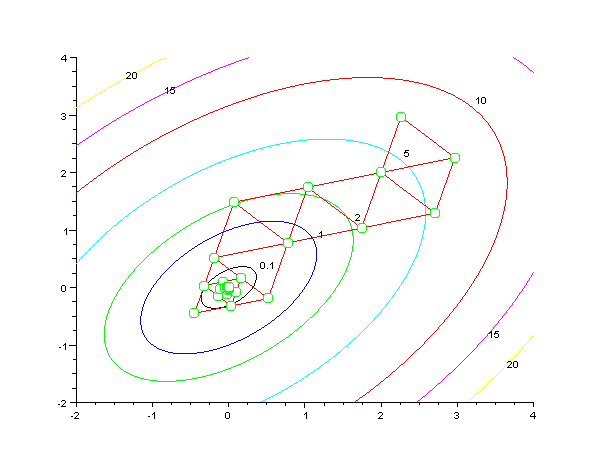
\includegraphics[width=15cm]{quad2bis-spendley-simplexcontours.png}
\end{center}
\caption{Spendley et al. numerical experiment -- History of simplex}
\label{fig-spendley-numexp1-historysimplex}
\end{figure}

The figure \ref{fig-spendley-numexp1-sigma} presents the history of the oriented
length of the simplex. The length is updated step by step, where each step 
corresponds to a shrink in the algorithm.

\begin{figure}
\begin{center}
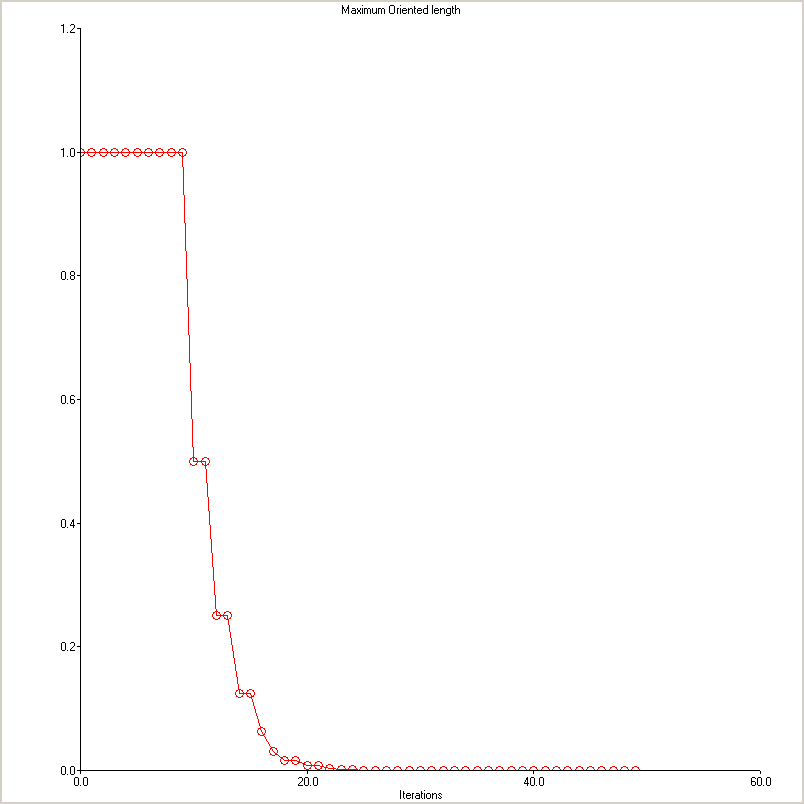
\includegraphics[width=10cm]{quad2bis-spendley-history-sigma.png}
\end{center}
\caption{Spendley et al. numerical experiment -- History of logarithm of the size of the simplex}
\label{fig-spendley-numexp1-sigma}
\end{figure}

The convergence is quite fast in this case, since less than 60 iterations
allow to get a function value lower than $10^{-15}$, as shown in 
figure \ref{fig-spendley-numexp1-logfopt}.

\begin{figure}
\begin{center}
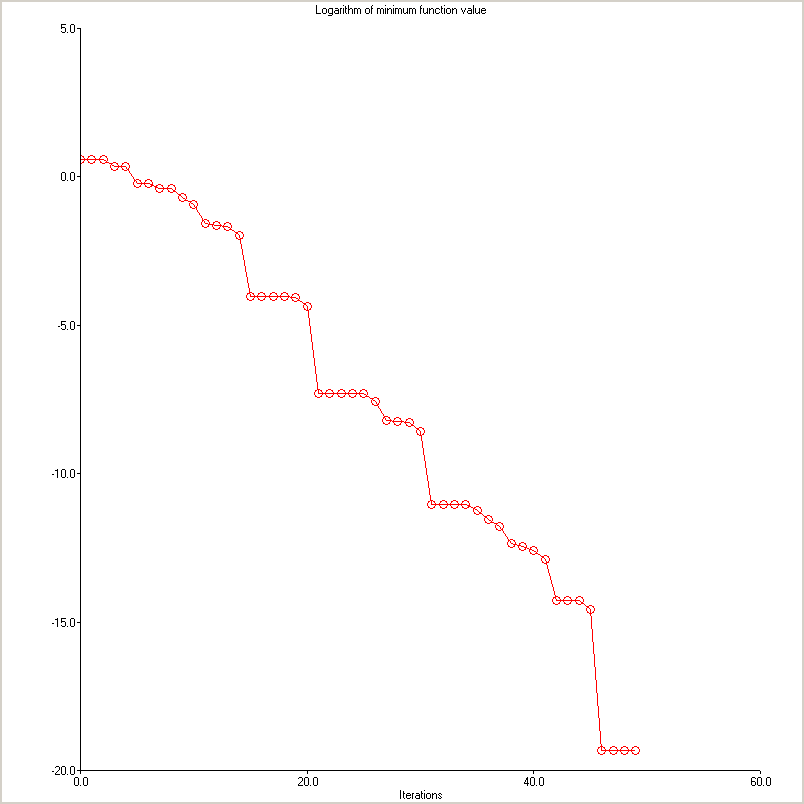
\includegraphics[width=10cm]{quad2bis-spendley-history-logfopt.png}
\end{center}
\caption{Spendley et al. numerical experiment -- History of logarithm of function}
\label{fig-spendley-numexp1-logfopt}
\end{figure}

\subsection{Badly scaled quadratic function}

The function we try to minimize is the following quadratic 
in 2 dimensions 
\begin{eqnarray}
\label{quadratic-sp-function2}
f(x_1,x_2) = a x_1^2 + x_2^2,
\end{eqnarray}
where $a>0$ is a chosen scaling parameter. 
The more $a$ is large, the more difficult the problem is 
to solve with the simplex algorithm.

We set the maximum number of function evaluations to 400.
The initial simplex is a regular simplex with length unity.

The following Scilab script uses the neldermead algorithm to perform the 
optimization.

\lstset{language=scilabscript}
\begin{lstlisting}
function y = quadratic (x)
  y = 100 * x(1)^2 + x(2)^2;
endfunction
nm = nmplot_new ();
nm = nmplot_configure(nm,"-numberofvariables",2);
nm = nmplot_configure(nm,"-function",quadratic);
nm = nmplot_configure(nm,"-x0",[10.0 10.0]');
nm = nmplot_configure(nm,"-maxiter",400);
nm = nmplot_configure(nm,"-maxfunevals",400);
nm = nmplot_configure(nm,"-tolxmethod","disabled");
nm = nmplot_configure(nm,"-tolsimplexizerelative",1.e-8);
nm = nmplot_configure(nm,"-simplex0method","spendley");
nm = nmplot_configure(nm,"-method","fixed");
nm = nmplot_configure(nm,"-verbose",1);
nm = nmplot_configure(nm,"-verbosetermination",0);
nm = nmplot_configure(nm,"-simplexfn","rosenbrock.fixed.history.simplex.txt");
nm = nmplot_configure(nm,"-fbarfn","rosenbrock.fixed.history.fbar.txt");
nm = nmplot_configure(nm,"-foptfn","rosenbrock.fixed.history.fopt.txt");
nm = nmplot_configure(nm,"-sigmafn","rosenbrock.fixed.history.sigma.txt");
nm = nmplot_search(nm);
nmplot_display(nm);
nm = nmplot_destroy(nm);
\end{lstlisting}


The numerical results are presented in table \ref{fig-spendley-numexp1-table},
where the experiment is presented for $a=100$. One can check that the 
number of function evaluation is equal to its maximum limit, even if the value of the 
function at optimum is very inacurate ($f(x^\star) \approx 0.08$).

\begin{figure}[h]
\begin{center}
\begin{tiny}
\begin{tabular}{|l|l|}
\hline
Iterations & 340 \\
Function Evaluations & 400 \\
$a$ & $100.0$ \\
$x_0$ & $(10.0,10.0)$ \\
Relative tolerance on simplex size & $10^{-8}$ \\
Exact $x^\star$ & $(0.,0.)$\\
Computed $x^\star$ & $(0.001,0.2)$\\
Computed $f(x^\star)$ & $0.08$\\
\hline
\end{tabular}
\end{tiny}
\end{center}
\caption{Numerical experiment with Spendley's et al. method on a badly scaled quadratic function}
\label{fig-spendley-numexp2-table}
\end{figure}


The various simplices generated during the iterations are 
presented in figure \ref{fig-spendley-numexp2-historysimplex}.
The method use reflections in the early iterations. Then there
is no possible improvment using reflections and shrinking is necessary.
But the shrinking makes the simplex very small so that a large number of 
iterations are necessary to improve the function value.
This is a limitation of the method, which is based on a simplex 
which can vary its size, but not its shape.

\begin{figure}
\begin{center}
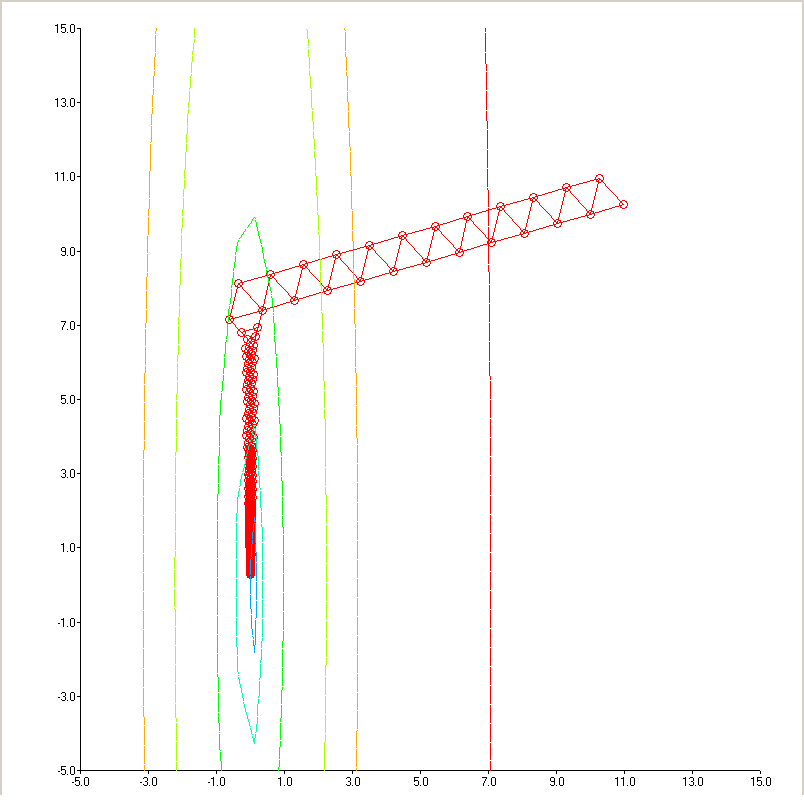
\includegraphics[width=15cm]{quad2-spendley-simplexcontours.png}
\end{center}
\caption{Spendley et al. numerical experiment with $f(x_1,x_2) = a x_1^2 + x_2^2$ and $a=100$ -- History of simplex}
\label{fig-spendley-numexp2-historysimplex}
\end{figure}

In figure \ref{fig-spendley-numexp2-scaling}, we analyse the 
behaviour of the method with respect to scaling.
We check that the method behave poorly when the scaling is 
bad. The convergence speed is slower and slower and impractical 
when $a>10$

\begin{figure}[htbp]
\begin{center}
\begin{tiny}
\begin{tabular}{|l|l|l|}
\hline
$a$ & Function evaluations & Computed $f(x^\star)$ \\
$1.0$ & 160 & $2.35e-18$ \\
$10.0$ & 222 & $1.2e-17$ \\
$100.0$ & 400 & $0.083$ \\
$1000.0$ & 400 & $30.3$ \\
$10000.0$ & 400 & $56.08$ \\
\hline
\end{tabular}
\end{tiny}
\end{center}
\caption{Numerical experiment with Spendley's et al. method on a badly scaled quadratic function}
\label{fig-spendley-numexp2-scaling}
\end{figure}

\subsection{Sensitivity to dimension}

In this section, we try to study the convergence of the 
Spendley et al. algorithm with respect to the number of variables.
The function we try to minimize is the following quadratic function 
in $n$-dimensions 
\begin{eqnarray}
\label{quadratic-sp-function3}
f(\bx) = \sum_{i=1,n} x_i^2.
\end{eqnarray}

The initial guess is at 0 so that this vertex is never updated 
during the iterations.
The initial simplex is computed with a random number generator.
The first vertex of the initial simplex is the origin.
The other vertices are uniform in the $[-1,1]$ interval.
for $i = 2, 2, \ldots , n+1$.
An absolute termination criteria on the size of the simplex is used.
More precisely, the method was stopped when $\sigma(Sk) \leq 10^{-8}$ is satisfied.

For this test, we compute the rate of convergence as presented
in Han \& Neuman \cite{HanNeumann2006}. This rate is defined as 
\begin{eqnarray}
\label{rho-sp-rate-convergence}
\rho(S_0,n) = \textrm{lim sup}_{k\rightarrow \infty} 
\left(\prod_{i=0,k-1} \frac{\sigma(S_{i+1})}{\sigma(S_i)}\right)^{1/k},
\end{eqnarray}
where $k$ is the number of iterations.
That definition can be viewed as the geometric mean of the ratio of the 
oriented lengths between successive simplices and the minimizer 0.
This definition implies 
\begin{eqnarray}
\label{rho-sp-rate-convergence2}
\rho(S_0,n) = \textrm{lim sup}_{k\rightarrow \infty} 
\left(\frac{\sigma(S_k)}{\sigma(S_0)}\right)^{1/k},
\end{eqnarray}

If $k$ is the number of iterations required to obtain convergence, as 
indicated by the termination criteria, the rate of convergence is practically computed as 
\begin{eqnarray}
\rho(S_0,n,k) = \left( \frac{\sigma(S_{k})}{\sigma(S_0)}\right)^{1/k}
\end{eqnarray}


\lstset{language=scilabscript}
\begin{lstlisting}
function y = quadratic (x)
  y = x(:).' * x(:);
endfunction
//
// myoutputcmd --
//  This command is called back by the Nelder-Mead
//  algorithm.
// Arguments
//  state : the current state of the algorithm
//    "init", "iter", "done"
//  data : the data at the current state
//    This is a tlist with the following entries:
//    * x : the optimal vector of parameters
//    * fval : the minimum function value
//    * simplex : the simplex, as a simplex object
//    * iteration : the number of iterations performed
//    * funccount : the number of function evaluations
//    * step : the type of step in the previous iteration
//
function myoutputcmd ( state , data , step )
  global STEP_COUNTER
  STEP_COUNTER(step) = STEP_COUNTER(step) + 1
endfunction

// OptimizeHanNeumann --
//   Perform the optimization and returns the object
// Arguments 
//   N : the dimension
function nm = OptimizeHanNeumann ( N )
  global STEP_COUNTER
  STEP_COUNTER("init") = 0;
  STEP_COUNTER("done") = 0;
  STEP_COUNTER("reflection") = 0;
  STEP_COUNTER("expansion") = 0;
  STEP_COUNTER("insidecontraction") = 0;
  STEP_COUNTER("outsidecontraction") = 0;
  STEP_COUNTER("expansion") = 0;
  STEP_COUNTER("shrink") = 0;
  STEP_COUNTER("reflectionnext") = 0;

  x0 = zeros(N,1);
  nm = neldermead_new ();
  nm = neldermead_configure(nm,"-numberofvariables",N);
  nm = neldermead_configure(nm,"-function",quadratic);
  nm = neldermead_configure(nm,"-x0",x0);
  nm = neldermead_configure(nm,"-maxiter",10000);
  nm = neldermead_configure(nm,"-maxfunevals",10000);
  nm = neldermead_configure(nm,"-tolxmethod","disabled");
  nm = neldermead_configure(nm,"-tolsimplexizeabsolute",1.e-8);
  nm = neldermead_configure(nm,"-tolsimplexizerelative",0);
  nm = neldermead_configure(nm,"-simplex0method","given");
  coords0(1,1:N) = zeros(1,N);
  coords0(2:N+1,1:N) = 2 * rand(N,N) - 1;
  nm = neldermead_configure(nm,"-coords0",coords0);
  nm = neldermead_configure(nm,"-method","fixed");
  nm = neldermead_configure(nm,"-verbose",0);
  nm = neldermead_configure(nm,"-verbosetermination",0);
  nm = neldermead_configure(nm,"-outputcommand",myoutputcmd);
  //
  // Perform optimization
  //
  nm = neldermead_search(nm);
endfunction

for N = 1:10
  nm = OptimizeHanNeumann ( N );
  niter = neldermead_get ( nm , "-iterations" );
  funevals = neldermead_get ( nm , "-funevals" );
  simplex0 = neldermead_get ( nm , "-simplex0" );
  sigma0 = optimsimplex_size ( simplex0 , "sigmaplus" );
  simplexopt = neldermead_get ( nm , "-simplexopt" );
  sigmaopt = optimsimplex_size ( simplexopt , "sigmaplus" );
  rho = ( sigmaopt / sigma0 ) ^ ( 1 / niter );
  //mprintf ( "%d %d %d %e\n" , N , funevals , niter , rho );
  mprintf("%d %s\n",N, strcat(string(STEP_COUNTER)," "))
  nm = neldermead_destroy(nm);
end

\end{lstlisting}

The figure \ref{fig-sp-numexp3-nbsteps} presents the type of 
steps which are performed for each number of variables.
We see that the algorithm mostly performs shrink steps.

\begin{figure}[htbp]
\begin{center}
\begin{tiny}
\begin{tabular}{|l|l|l|l|l|}
\hline
$n$ & \#Iterations & \# Reflections & \# Reflection & \#Shrink\\
 & & / High & / Next to High & \\
\hline
1 & 27 & 0 & 0 & 26\\
2 & 28 & 0 & 0 & 27\\
3 & 30 & 2 & 0 & 27\\
4 & 31 & 1 & 1 & 28\\
5 & 29 & 0 & 0 & 28\\
6 & 31 & 2 & 0 & 28\\
7 & 29 & 0 & 0 & 28\\
8 & 29 & 0 & 0 & 28\\
9 & 29 & 0 & 0 & 28\\
10 & 29 & 0 & 0 & 28\\
11 & 29 & 0 & 0 & 28\\
12 & 29 & 0 & 0 & 28\\
13 & 31 & 0 & 2 & 28\\
14 & 29 & 0 & 0 & 28\\
15 & 29 & 0 & 0 & 28\\
16 & 31 & 0 & 1 & 29\\
17 & 30 & 0 & 0 & 29\\
18 & 30 & 0 & 0 & 29\\
19 & 31 & 0 & 1 & 29\\
20 & 32 & 2 & 0 & 29\\
\hline
\end{tabular}
\end{tiny}
\end{center}
\caption{Numerical experiment with Spendley et al method on a generalized quadratic function -- number 
and kinds of steps performed}
\label{fig-sp-numexp3-nbsteps}
\end{figure}

The figure \ref{fig-sp-numexp3-dimension} presents the number of function 
evaluations depending on the number of variables.

One can see that the number of function evaluations 
increases approximately linearily with the dimension of the problem in
figure \ref{fig-sp-numexp3-fvn}. A rough rule of thumb is that, for $n=1,20$, 
the number of function evaluations is equal to $30n$.
This test is in fact the best that we can expect from this algorithm : since 
most iterations are shrink steps, most iterations improves the function value.

\begin{figure}[htbp]
\begin{center}
\begin{tiny}
\begin{tabular}{|l|l|l|l|}
\hline
$n$ & Function  & Iterations & $\rho(S_0,n)$\\
    & Evaluations &          & \\
\hline
1 & 81 & 27 & 0.513002 \\
2 & 112 & 28 & 0.512532 \\
3 & 142 & 29 & 0.524482 \\
4 & 168 & 28 & 0.512532 \\
5 & 206 & 31 & 0.534545 \\
6 & 232 & 29 & 0.512095 \\
7 & 262 & 30 & 0.523127 \\
8 & 292 & 30 & 0.523647 \\
9 & 321 & 30 & 0.523647 \\
10 & 348 & 29 & 0.512095 \\
11 & 377 & 29 & 0.512095 \\
12 & 406 & 29 & 0.512095 \\
13 & 435 & 29 & 0.512095 \\
14 & 464 & 29 & 0.512095 \\
15 & 493 & 29 & 0.512095 \\
16 & 540 & 30 & 0.511687 \\
17 & 570 & 30 & 0.511687 \\
18 & 600 & 30 & 0.511687 \\
19 & 630 & 30 & 0.511687 \\
20 & 660 & 30 & 0.511687 \\
\hline
\end{tabular}
\end{tiny}
\end{center}
\caption{Numerical experiment with Spendley et al. method on a generalized quadratic function}
\label{fig-sp-numexp3-dimension}
\end{figure}

\begin{figure}
\begin{center}
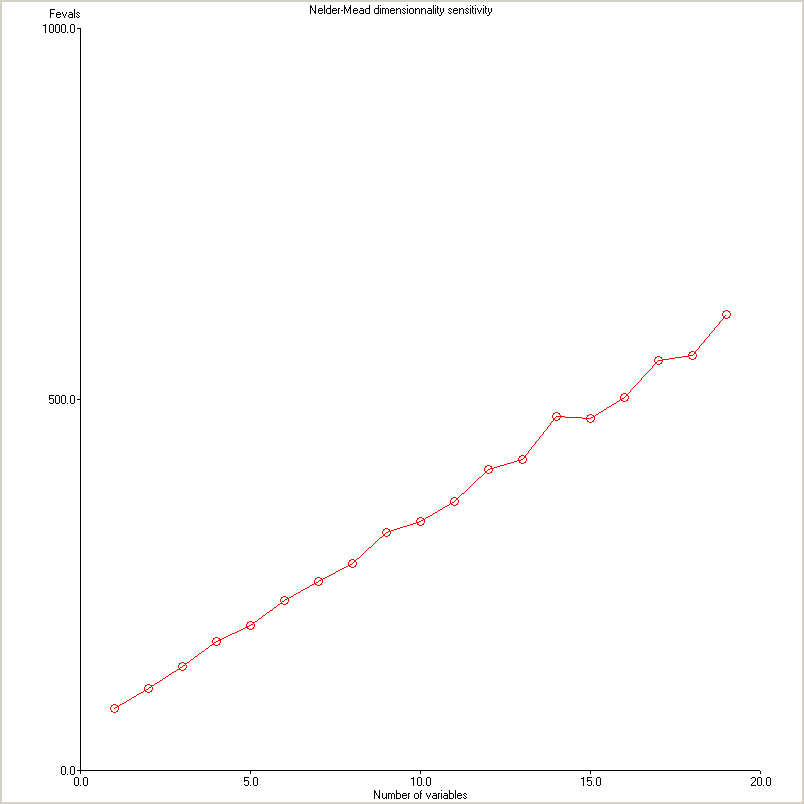
\includegraphics[width=10cm]{spendley-dimension-nfevals.png}
\end{center}
\caption{Spendley et al. numerical experiment -- Number of function evaluations 
depending on the number of variables}
\label{fig-sp-numexp3-fvn}
\end{figure}

The table \ref{fig-sp-numexp3-dimension} also shows the interesting 
fact that the convergence rate is almost constant and 
very close to 1. This is a consequence of the shrink steps,
which are dividing the size of the simplex at each iterations by 2.
Therefore, the convergence rate is close to $1/2$.

\section{Conclusion}

We saw in the first numerical experiment that the method 
behave reasonably when the function is correctly scaled.
When the function is badly scaled, as in the second numerical 
experiment, the Spendley et al. algorithm produces a large 
number of function evaluations and converges very slowly.
This limitation occurs with even moderate badly scaled 
functions and generates a very slow method in these 
cases.

In the last experiment, we have explored what happens when the number of 
iterations is increasing. The rate of convergence in this case is close to $1/2$
and the number of function evaluations is a linear function of the number 
of variables (approximately $30n$ in this case).

